As implemented for \dword{pdsp}, a fully loaded \dword{wib} (one \dword{wib} plus four \dwords{femb}) requires
\SI{12}{V} and draws up to approximately \SI{4}{A}. The full electronics for one \dword{apa} (one \dword{ptc}, five \dwords{wib}, and \num{20} \dwords{femb}) 
requires \SI{12}{V} and draws approximately \SI{20}{A}, for a total power of approximately \SI{240}{W}, as 
described in Section~\ref{sec:fdsp-tpc-elec-design-warm}. The \dword{spmod} implementation should require much 
less power as the \dword{fpga} will be replaced by the \dword{coldata} chips.

As the \dword{lv} power is delivered at \SI{48}{V} to the \dword{ptc}, each \dword{lv} power mainframe is chosen to bracket that value; each has  
roughly \numrange{30}{60}{V}, \SI{13.5}{A}, \SI{650}{W} maximum capacity per \dword{apa}. Using 10AWG cable, a \SI{0.8}{V} drop is 
expected along the cable with a required power of \SI{306}{W} out of \SI{650}{W} available.  
This leaves a significant margin that allows for larger distances between the power supplies and 
the warm interface crates than the \SI{20}{\meter} in \dword{pdsp}.

Four wires are used for each module; two 10AWG, shielded, twisted-pair cables for the power and return; and two 20AWG, shielded, twisted-pair cables for the sense.
The primary protection is the over-current protection circuit in the \dword{lv} supply modules, 
which is set above the \SI{20}{A} current draw of the \dword{wiec}.  Secondary sense line fusing is 
provided on the \dword{ptc}.  The \dword{lv} power cable uses FCi micro TCA\footnote{MicroTCA\texttrademark{} (\dword{utca}) vertical card-edge connectors, Amphenol ICC,  \url{https://www.amphenol-icc.com/product-series/micro-tca-card-edge.html}.} connectors, shown in
Figure~\ref{fig:tpcelec-power_conn}.

\begin{dunefigure}
[FCi micro TCA power connector at the \dword{ptc} end of the cable.]
{fig:tpcelec-power_conn}
{FCi micro TCA power connector at the \dword{ptc} end of the cable.}
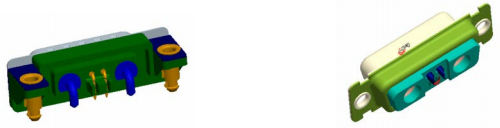
\includegraphics[width=0.9\linewidth]{tpcelec-power_connector.png}
\end{dunefigure}

Bias voltages for the \dword{apa} wire planes, the electron diverters, and the last \dword{fc} electrodes are generated by supplies which are the responsibility of the TPC Electronics consortium.  The current from each of these supplies is expected to be very close to zero in normal operation.  However, the ripple voltage must be carefully controlled to avoid injecting noise into the front-end electronics.  RG-58 coaxial cables connect the wire bias voltages from the mini-crate to the standard SHV
connectors machined directly into the \dword{ce} \fdth, so there is no electrical connection between 
the \dword{lv} power and data connectors and wire bias voltages.

Optical fibers are used for all connections between the \dwords{wiec}, which act as
Faraday-shielded boxes, and the \dword{daq} and slow control systems.  %Duplex LC optical fiberstransmit the one GIG-E connection from each \dword{wib} to the slow control system.  
The \dword{wib} reports
its onboard temperature and the current draw from each \dword{femb} to the slow control system, while the
current draw for each \dword{apa} is monitored at the mainframe itself.
